\section{Background}
\label{background}

The Python programming language~\cite{pythonlang} was designed by Guido van Rossum in the early 1990s as a descendant of the ABC programming language, which was a teaching language created by van Rossum in the early 1980s.  It includes a sizeable standard library, powerful primitive data types, and a self-documenting system based on the language's emphasis on readability of source text.  It is interpreted by a few different programs.

C-Python~\cite{python}, currently the most widely used interpreter for the Python programming language, is implemented in the C language.  Another Python interpreter, Jython~\cite{jython}, is written in Java.  The compiler this paper describes serves as yet another interpreter; it is written in MzScheme.

MzScheme~\cite{mzscheme} is an interpreter for the MzScheme programming language~\cite{mzschemelang}, which is a dialect of the Scheme language~\cite{kelsey98revised}.  MzScheme compiles syntactically valid MzScheme language programs into the MzScheme Core language, a subset of the MzScheme language, before compiling the core language into an internal bytecode representation for evaluation.

MrEd~\cite{mred} is a graphical user interface (GUI) toolkit that builds on the MzScheme interpreter and works uniformally across several platforms, namely Windows, Mac OS X, and the X Window System.

\begin{figure}
	\caption{PLT Scheme partial language hierarchy}
	\label{schemelanguagesfig}
	\begin{center}
		\includegraphics{images/scheme-languages}
	\end{center}
\end{figure}


Originally meant for Scheme, DrScheme~\cite{bruce97drscheme} is an integrated development environment (IDE) based on MzScheme---it is a MrEd application---with support for embedding third-party extensions.  DrScheme provides developers with useful and modular development tools, such as syntax or flow analyzers, which accept the MzScheme Core language as their input.  Because the internal DrScheme data structures representing MzScheme code also store source file location, any reference by a development tool or the MzScheme interpreter to the Core code can be mapped back to a reference to the original program text.

DrScheme is no longer a development environment only for Scheme.  It can now potentially play the role of a program development environment for any language, which users can select from a menu (Figure~\ref{drschemelangmenufig}).  When using any language from within the IDE, the program developer may use all of DrScheme's development tools, such as Syntax Check, which checks a program's syntax and highlights its bindings (Figure~\ref{syntaxcheckschemefig}), or MrFlow, which analyses a program's possible flow of values.  Also, any new tool added to the DrScheme IDE will automatically work with all languages that DrScheme now supports (Figure~\ref{syntaxcheckpythonfig}).

\begin{figure}
	\caption{DrScheme language selection menu}
	\label{drschemelangmenufig}
	\begin{center}
		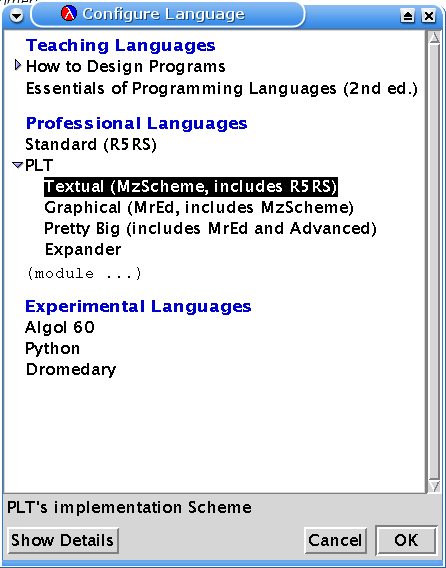
\includegraphics{images/drscheme-lang-menu}
	\end{center}
\end{figure}

To support a new language, however, DrScheme needs software to translate programs written in the new language into MzScheme.  In the case of adding Python support to DrScheme, this is the task of the Python-to-Scheme compiler.  The compiler is packaged as a DrScheme language tool, thus introducing Python as a language in DrScheme's graphical list of choices (Figure~\ref{drschemelangmenufig}).  This paper describes the components that comprise the compiler.  Section~\ref{grammar} presents the Python grammar used in this implementation.  Section~\ref{implementation} describes the implementation itself.

\begin{figure}
	\caption{Syntax Check and Scheme}
	\label{syntaxcheckschemefig}
	\begin{center}
		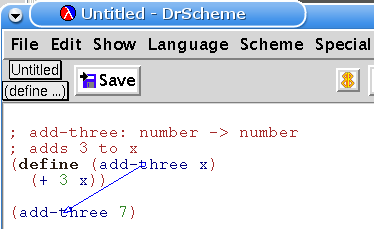
\includegraphics{images/syntax-check-scheme}
	\end{center}
\end{figure}

\begin{figure}
	\caption{Syntax Check and Python}
	\label{syntaxcheckpythonfig}
	\begin{center}
		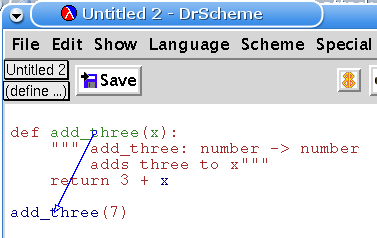
\includegraphics{images/syntax-check-python}
	\end{center}
\end{figure}
